\documentclass[tikz,border=8pt]{standalone}
\usepackage{amsmath}
\usepackage{amssymb}
\usepackage{tikz}
\usetikzlibrary{arrows.meta,calc,decorations.pathreplacing,patterns,shapes.geometric,positioning,shadings,plotmarks}

\begin{document}
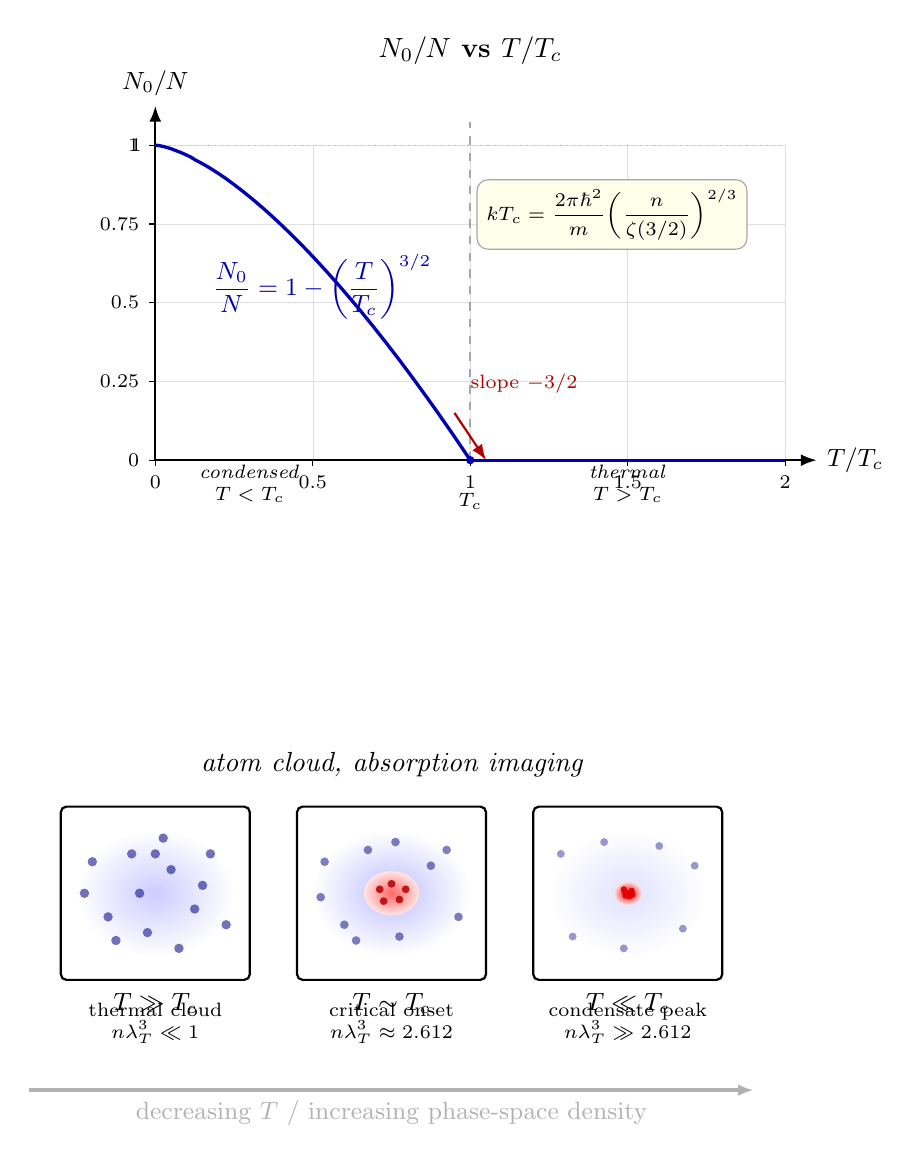
\begin{tikzpicture}[
    >={Latex[length=2mm]},
    font=\small
]

% =============================================
% TOP: Condensate fraction curve N0/N vs T/Tc
% =============================================
\begin{scope}[shift={(0,4)}]
  % Axes
  \def\xmax{2.0}
  \def\xscale{4.0}  % cm per (T/Tc)
  \def\yscale{4.0}  % cm per (N0/N)

  % Grid
  \draw[very thin, gray!25] (0,0) grid[xstep=0.5*\xscale, ystep=0.25*\yscale] (\xmax*\xscale,1*\yscale);

  % Axes lines
  \draw[->, thick] (0,0) -- (\xmax*\xscale+0.4,0) node[right] {$T/T_c$};
  \draw[->, thick] (0,0) -- (0,1*\yscale+0.5) node[above] {$N_0/N$};

  % X tick labels
  \foreach \x/\lab in {0/0, 0.5/0.5, 1/1, 1.5/1.5, 2/2}
    \draw (\x*\xscale,0) -- (\x*\xscale,-0.08) node[below] {\scriptsize \lab};

  % Y tick labels
  \foreach \y/\lab in {0/0, 0.25/0.25, 0.5/0.5, 0.75/0.75, 1/1}
    \draw (0,\y*\yscale) -- (-0.08,\y*\yscale) node[left] {\scriptsize \lab};

  % Vertical dashed line at T=Tc
  \draw[dashed, thick, gray!70] (1*\xscale,0) -- (1*\xscale,1*\yscale+0.3);
  \node[below] at (1*\xscale,-0.3) {\scriptsize $T_c$};

  % Horizontal at N0/N=1
  \draw[dotted, gray!60] (0,1*\yscale) -- (\xmax*\xscale,1*\yscale);
  \node[left] at (-0.05,1*\yscale) {\scriptsize $1$};

  % Curve for T<Tc: N0/N = 1 - (T/Tc)^{3/2}
  \draw[very thick, blue!70!black, smooth, samples=80, domain=0:1]
       plot (\x*\xscale, {(1 - pow(\x,1.5))*\yscale});

  % Curve for T>=Tc: N0/N = 0
  \draw[very thick, blue!70!black] (1*\xscale,0) -- (\xmax*\xscale,0);

  % Marker dot at Tc
  \fill[blue!70!black] (1*\xscale,0) circle (1.5pt);

  % Title
  \node[above, font=\bfseries] at (\xmax*\xscale/2, 1*\yscale+0.9)
        {$N_0/N$ vs $T/T_c$};

  % Curve equation label
  \node[blue!70!black, anchor=west] at (0.15*\xscale, 0.55*\yscale)
        {\small $\dfrac{N_0}{N}=1-\left(\dfrac{T}{T_c}\right)^{3/2}$};

  % Tc formula box (below curve, right side)
  \node[draw=gray!70, fill=yellow!8, rounded corners, align=left, font=\scriptsize]
       at (1.45*\xscale, 0.78*\yscale)
       {$kT_c=\dfrac{2\pi\hbar^2}{m}\!\left(\dfrac{n}{\zeta(3/2)}\right)^{2/3}$};

  % Annotate phases
  \node[align=center, font=\scriptsize] at (0.3*\xscale, 0.05*\yscale-0.5)
        {\textit{condensed}\\ $T<T_c$};
  \node[align=center, font=\scriptsize] at (1.5*\xscale, 0.05*\yscale-0.5)
        {\textit{thermal}\\ $T>T_c$};

  % Slope -3/2 indicator near Tc
  \draw[red!70!black, thick, ->] (0.95*\xscale, 0.15*\yscale) -- (1.05*\xscale, 0.0*\yscale);
  \node[red!70!black, font=\scriptsize, anchor=south west]
       at (0.97*\xscale, 0.18*\yscale) {slope $-3/2$};

\end{scope}

% =============================================
% BOTTOM: Three atom cloud cartoons
% =============================================
\begin{scope}[shift={(0,-1.5)}]

  \def\boxw{2.4}
  \def\boxh{2.2}
  \def\sep{0.6}

  % --- Panel 1: T >> Tc (thermal cloud, broad, uniform) ---
  \begin{scope}[shift={(0,0)}]
    \draw[thick, rounded corners=2pt] (-\boxw/2,-\boxh/2) rectangle (\boxw/2,\boxh/2);
    % Background gradient cloud (broad, low contrast)
    \shade[inner color=blue!20, outer color=white]
          (0,0) ellipse (1.0 and 0.8);
    % Random thermal atoms
    \foreach \x/\y in {-0.8/0.4, -0.6/-0.3, -0.3/0.5, -0.1/-0.5, 0.2/0.3,
                       0.5/-0.2, 0.7/0.5, 0.9/-0.4, -0.9/0.0, 0.1/0.7,
                       -0.5/-0.6, 0.6/0.1, -0.2/0.0, 0.3/-0.7, 0.0/0.5}{
      \fill[blue!50!black, opacity=0.55] (\x,\y) circle (0.06);
    }
    \node[below] at (0,-\boxh/2-0.05) {$T\gg T_c$};
    \node[font=\scriptsize, align=center] at (0,-\boxh/2-0.55)
         {thermal cloud\\ $n\lambda_T^3 \ll 1$};
  \end{scope}

  % --- Panel 2: T ~ Tc (critical: small dense core forming) ---
  \begin{scope}[shift={(\boxw+\sep,0)}]
    \draw[thick, rounded corners=2pt] (-\boxw/2,-\boxh/2) rectangle (\boxw/2,\boxh/2);
    % Outer thermal cloud
    \shade[inner color=blue!25, outer color=white]
          (0,0) ellipse (1.0 and 0.8);
    % Inner forming peak
    \shade[inner color=red!60, outer color=red!10]
          (0,0) ellipse (0.35 and 0.28);
    % Atoms
    \foreach \x/\y in {-0.85/0.4, -0.6/-0.4, -0.3/0.55, 0.1/-0.55, 0.5/0.35,
                       0.85/-0.3, 0.7/0.55, -0.9/-0.05, 0.05/0.65, -0.45/-0.6}{
      \fill[blue!50!black, opacity=0.5] (\x,\y) circle (0.055);
    }
    \foreach \x/\y in {-0.15/0.05, 0.1/-0.08, 0.0/0.12, 0.18/0.05, -0.1/-0.1}{
      \fill[red!70!black, opacity=0.85] (\x,\y) circle (0.05);
    }
    \node[below] at (0,-\boxh/2-0.05) {$T\sim T_c$};
    \node[font=\scriptsize, align=center] at (0,-\boxh/2-0.55)
         {critical onset\\ $n\lambda_T^3 \approx 2.612$};
  \end{scope}

  % --- Panel 3: T << Tc (sharp condensate peak, sparse thermal halo) ---
  \begin{scope}[shift={(2*\boxw+2*\sep,0)}]
    \draw[thick, rounded corners=2pt] (-\boxw/2,-\boxh/2) rectangle (\boxw/2,\boxh/2);
    % Faint thermal halo
    \shade[inner color=blue!12, outer color=white]
          (0,0) ellipse (1.0 and 0.8);
    % Sharp condensate peak (about 1/6 the size of halo)
    \shade[inner color=red!85!black, outer color=red!10]
          (0,0) ellipse (0.18 and 0.15);
    % Sparse halo atoms
    \foreach \x/\y in {-0.85/0.5, 0.7/-0.45, -0.3/0.65, 0.85/0.35, -0.7/-0.55,
                       0.4/0.6, -0.05/-0.7}{
      \fill[blue!50!black, opacity=0.4] (\x,\y) circle (0.05);
    }
    % Dense condensate atoms
    \foreach \x/\y in {0/0, 0.05/0.03, -0.04/0.02, 0.02/-0.04, -0.03/-0.03,
                       0.06/-0.02, -0.05/0.05}{
      \fill[red!90!black, opacity=0.95] (\x,\y) circle (0.04);
    }
    \node[below] at (0,-\boxh/2-0.05) {$T\ll T_c$};
    \node[font=\scriptsize, align=center] at (0,-\boxh/2-0.55)
         {condensate peak\\ $n\lambda_T^3 \gg 2.612$};
  \end{scope}

  % Section label
  \node[above, font=\itshape] at (\boxw+\sep, \boxh/2+0.25)
       {atom cloud, absorption imaging};

  % Arrow indicating cooling direction
  \draw[->, very thick, gray!60] (-\boxw/2-0.4, -\boxh/2-1.4) --
        (2*\boxw+2*\sep+\boxw/2+0.4, -\boxh/2-1.4)
        node[midway, below, font=\small] {decreasing $T$ / increasing phase-space density};

\end{scope}

\end{tikzpicture}
\end{document}
